\chapter{De levende wereld indelen}\label{ch:b1:classifying-biodiversity}

Er zijn ongeveer \num{2} miljoen \omterm{def:b1:classifying-biodiversity:species}{soorten} benoemd, en elk jaar komen er zo'n
\num{18000} bij; het aantal dat bestaat wordt alleen al voor de eukaryoten op
bijna \num{9} miljoen geschat, en niemand weet hoeveel bacteriën er zijn. Een
naam is pas het begin: een bioloog wil weten welke \omterm{def:b1:classifying-biodiversity:species}{soort} het dichtst bij welke
staat, en het antwoord is een boom, omdat de \omterm{def:b1:classifying-biodiversity:species}{soorten} door afstamming verwant
zijn. Dit hoofdstuk geeft de regels van de naamgeving, de methoden waarmee
verwantschappen uit kenmerken worden afgeleid --- en het criterium,
\omterm{def:b1:classifying-biodiversity:parsimony}{spaarzaamheid}, waarmee concurrerende bomen worden beoordeeld --- de vorm van
de levensboom zoals hij nu wordt begrepen, en de stand van de inventaris van
wat er leeft.

\section{Soorten en namen}

\begin{definition}[Soort]\label{def:b1:classifying-biodiversity:species}
\index{soort}\index{biologisch soortsbegrip}
Een \emph{soort} is, volgens het \emph{biologische soortsbegrip}, een groep
\omterm{def:b1:populations:population}{populaties} waarvan de leden zich onderling kunnen voortplanten en vruchtbare
nakomelingen krijgen en die voortplantingskundig van andere zulke groepen
zijn afgezonderd. Het begrip is niet toepasbaar op \omterm{def:b1:organism-environment:organism}{organismen} die zich niet
geslachtelijk voortplanten (de meeste bacteriën, veel protisten en sommige
planten en dieren), op fossielen, of op \omterm{def:b1:populations:population}{populaties} die elkaar nooit
ontmoeten; daar wordt een soort herkend aan haar bouw (het
\emph{morfologische} begrip), aan haar eigen tak op een boom (het
\emph{fylogenetische} begrip), of aan een drempel van genetisch verschil. Alle
begrippen proberen hetzelfde te benoemen: een lijn die zich apart van andere
ontwikkelt.
\end{definition}

\begin{definition}[Naamgeving en rangen]\label{def:b1:classifying-biodiversity:nomenclature}
\index{binomiale naamgeving}\index{taxon}\index{geslacht}\index{typemateriaal}
Elke \omterm{def:b1:classifying-biodiversity:species}{soort} heeft een \emph{binomiale} naam: de naam van haar
\emph{geslacht} (met hoofdletter) gevolgd door een soortaanduiding, beide
cursief --- \emph{Homo sapiens}, \emph{Quercus robur},
\emph{Escherichia coli} --- vaak gevolgd door de auteur en het jaar van de
beschrijving. Het stelsel, in 1753 (planten) en 1758 (dieren) door Linnaeus
vastgelegd, nestelt \omterm{def:b1:classifying-biodiversity:species}{soorten} in een hiërarchie van \emph{rangen}: geslacht,
familie, orde, klasse, stam (of afdeling), rijk, domein. Een groep op elke
rang heet een \emph{taxon}. Elke naam is gebonden aan een stuk
\emph{typemateriaal}, dat in een museum of herbarium wordt bewaard en
vastlegt waarnaar de naam verwijst; de oudste geldige naam heeft voorrang; en
de regels zijn zo vastgelegd dat één \omterm{def:b1:organism-environment:organism}{organisme} wereldwijd één naam heeft. De
rangen zijn afspraken --- er is geen eigenschap die alle families delen en
geen geslacht heeft; alleen de \omterm{def:b1:classifying-biodiversity:species}{soort} is een natuurlijke eenheid.
\end{definition}

\begin{omfigure}
\begin{tikzpicture}[font=\footnotesize, line cap=round]
  \draw[thick, omDef!60!black, fill=omDef!6, rounded corners=4pt] (0,0) rectangle (11.4,5.4); \node[anchor=north west, omDef!80!black] at (0.1,5.35) {domein Eukarya};
  \draw[thick, omDef!60!black, fill=omDef!10, rounded corners=4pt] (0.4,0.3) rectangle (11.0,4.75); \node[anchor=north west, omDef!80!black] at (0.5,4.7) {rijk Animalia};
  \draw[thick, omProp!70!black, fill=omProp!10, rounded corners=4pt] (0.8,0.6) rectangle (10.6,4.1); \node[anchor=north west, omProp!80!black] at (0.9,4.05) {stam Chordata};
  \draw[thick, omProp!70!black, fill=omProp!18, rounded corners=4pt] (1.2,0.9) rectangle (10.2,3.45); \node[anchor=north west, omProp!80!black] at (1.3,3.4) {klasse Mammalia};
  \draw[thick, omThm!70!black, fill=omThm!10, rounded corners=4pt] (1.6,1.2) rectangle (9.8,2.8); \node[anchor=north west, omThm!80!black] at (1.7,2.75) {orde Carnivora};
  \draw[thick, omThm!70!black, fill=omThm!20, rounded corners=4pt] (2.0,1.4) rectangle (5.6,2.3); \node[anchor=north west, omThm!80!black] at (2.1,2.25) {familie Felidae};
  \node[anchor=west] at (2.1,1.65) {geslacht \emph{Felis}: \emph{F.~catus}};
  \draw[thick, omThm!70!black, fill=omThm!20, rounded corners=4pt] (5.9,1.4) rectangle (9.5,2.3); \node[anchor=north west, omThm!80!black] at (6.0,2.25) {familie Canidae};
  \node[anchor=west] at (6.0,1.65) {geslacht \emph{Canis}: \emph{C.~lupus}};
\end{tikzpicture}

{\small De geneste rangen van de hiërarchie van Linnaeus, voor de kat en de
wolf. Elk vak is een \omterm{def:b1:classifying-biodiversity:nomenclature}{taxon}; de binomiale naam noemt het \omterm{def:b1:classifying-biodiversity:nomenclature}{geslacht} en de
\omterm{def:b1:classifying-biodiversity:species}{soort}.}
\end{omfigure}

\begin{omfigure}
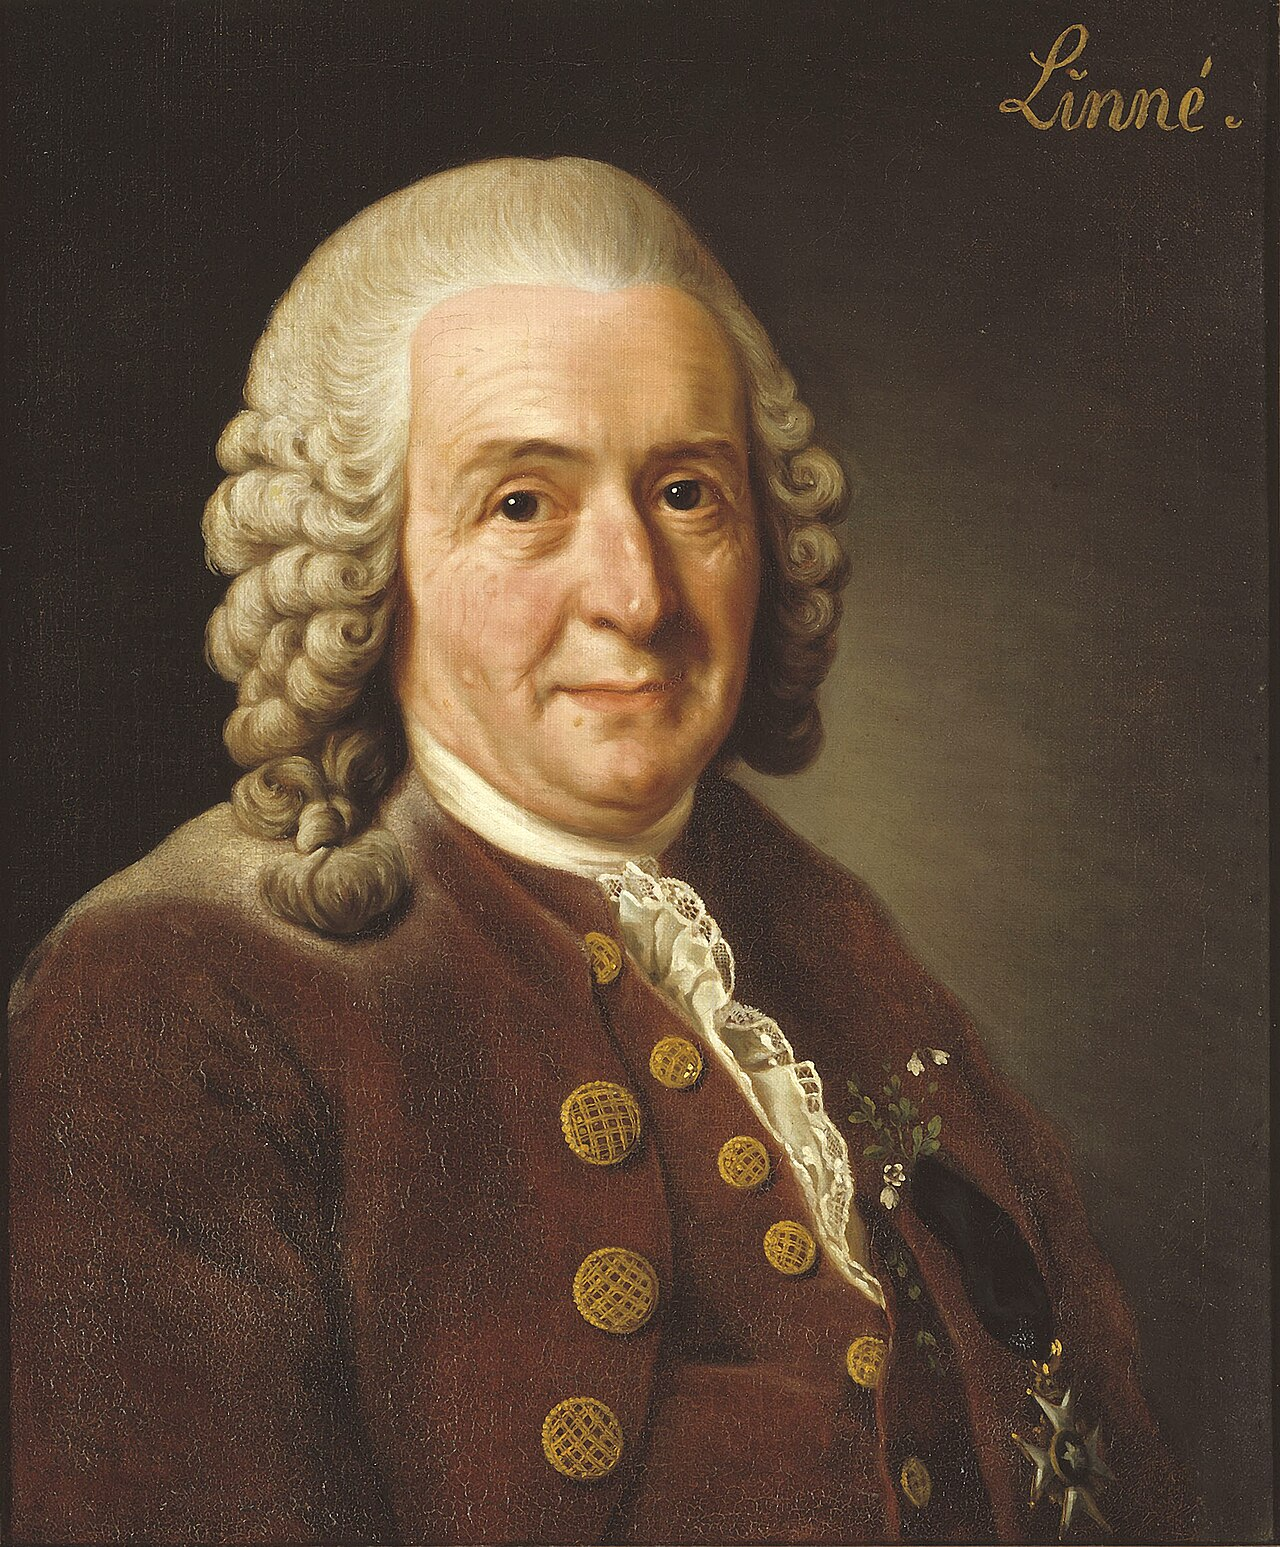
\includegraphics[width=0.36\linewidth]{images/book3/linnaeus.jpg}

{\small Carl Linnaeus (1707--1778), wiens \emph{Species Plantarum} van 1753
en tiende uitgave van de \emph{Systema Naturae} van 1758 de uitgangspunten
van de botanische en de zoölogische naamgeving zijn. Portret door Alexander
Roslin, 1775.}
\end{omfigure}

\begin{omfigure}
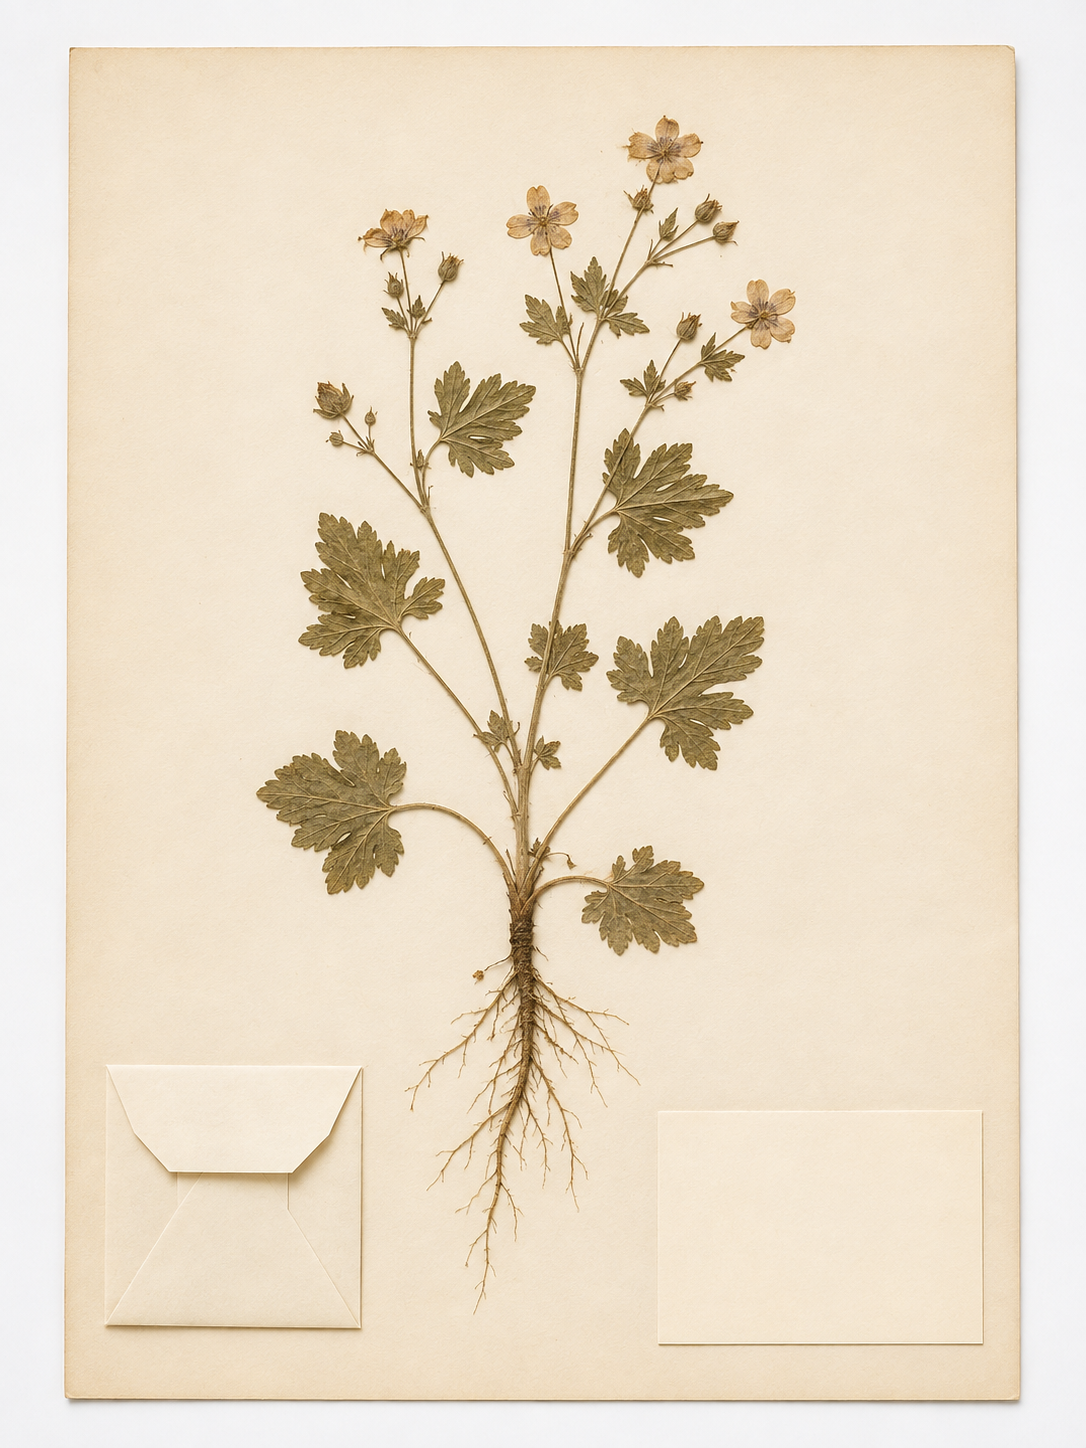
\includegraphics[width=0.5\linewidth]{images/book3/ai/b3-29-herbarium-sheet.png}

{\small Een herbariumblad: een geperst, van een etiket voorzien exemplaar
zoals dat als \omterm{def:b1:classifying-biodiversity:nomenclature}{typemateriaal} van een plantennaam dient en als het blijvende
bewijs van waar en wanneer de \omterm{def:b1:classifying-biodiversity:species}{soort} is gevonden.}
\end{omfigure}

\section{Verwantschappen reconstrueren}

\begin{definition}[Systematiek, fylogenie, cladistiek]\label{def:b1:classifying-biodiversity:systematics}
\index{systematiek}\index{fylogenie}\index{cladistiek}\index{clade}
\emph{Systematiek} is de studie van de verscheidenheid van \omterm{def:b1:organism-environment:organism}{organismen} en van
de verwantschappen daartussen; een \emph{fylogenie} is de boom van die
verwantschappen, een hypothese over de volgorde waarin de lijnen zich hebben
gesplitst. \emph{Fenetiek} groepeert \omterm{def:b1:organism-environment:organism}{organismen} naar hun algehele
gelijkenis en telt alle kenmerken even zwaar; \emph{cladistiek} groepeert ze
alleen naar gedeelde afgeleide kenmerken, zodat elke groep een \emph{clade}
is --- een voorouder met al zijn nakomelingen. De moderne indeling streeft
ernaar elk benoemd \omterm{def:b1:classifying-biodiversity:nomenclature}{taxon} een clade te laten zijn.
\end{definition}

\begin{definition}[Kenmerken: homologie, homoplasie, polariteit]\label{def:b1:classifying-biodiversity:characters}
\index{homologie}\index{homoplasie}\index{synapomorfie}\index{buitengroep}
Een \emph{kenmerk} is elke erfelijke eigenschap met twee of meer
\emph{toestanden} (ledemaat aanwezig of afwezig; een bepaalde base in een \omterm{def:b1:genomes:gene}{gen}
A, C, G of T). De kenmerken van twee \omterm{def:b1:organism-environment:organism}{organismen} zijn \emph{homoloog} wanneer
zij van een gemeenschappelijke voorouder zijn geërfd, \emph{homoplastisch}
wanneer zij gelijken door convergentie of terugkeer (de vleugels van vogels
en vleermuizen; de gestroomlijnde lichamen van dolfijnen en haaien). Een
kenmerktoestand is \emph{oorspronkelijk} (plesiomorf) als zij bij de
voorouder van de groep aanwezig was, \emph{afgeleid} (apomorf) als zij binnen
de groep is ontstaan; de afgeleide toestanden die een \omterm{def:b1:classifying-biodiversity:systematics}{clade} deelt, haar
\emph{synapomorfieën}, zijn het enige bewijs ervoor. De polariteit wordt
bepaald door vergelijking met een \emph{buitengroep}, een \omterm{def:b1:classifying-biodiversity:nomenclature}{taxon} waarvan
bekend is dat het buiten de bestudeerde groep ligt: de toestand die het
vertoont wordt als oorspronkelijk genomen.
\end{definition}

\begin{definition}[Monofylie, parafylie, polyfylie]\label{def:b1:classifying-biodiversity:monophyly}
\index{monofylie}\index{parafylie}\index{polyfylie}
Een groep is \emph{monofyletisch} (een \omterm{def:b1:classifying-biodiversity:systematics}{clade}) als zij een voorouder met al
zijn nakomelingen bevat; \emph{parafyletisch} als zij een voorouder en slechts
een deel van zijn nakomelingen bevat (de ``reptielen'', die de vogels
uitsluiten die van hen afstammen; de ``vissen'', die de viervoeters
uitsluiten; de ``ongewervelden''); \emph{polyfyletisch} als zij nakomelingen
van verschillende voorouders op grond van een convergent kenmerk samenbrengt
(de ``warmbloedige dieren'', vogels en zoogdieren; de ``algen'').
Parafyletische groepen zijn nuttige beschrijvingen van
\omterm{def:b1:organism-environment:levels}{organisatieniveaus} maar zijn geen \omterm{def:b1:classifying-biodiversity:systematics}{claden} en krijgen geen formele naam meer.
\end{definition}

\begin{omfigure}
\begin{tikzpicture}[font=\footnotesize, line cap=round, >=Stealth]
  % tree: lamprey, shark, trout, lungfish, frog, lizard, bird, mammal
  \coordinate (r) at (6.5,-1.2);
  \draw[thick] (r) -- (6.5,-0.2);
  \draw[thick] (6.5,-0.2) -- (0.5,-0.2) -- (0.5,4.6); \node[anchor=south, rotate=60, anchor=west] at (0.5,4.6) {prik};
  \draw[thick] (6.5,-0.2) -- (6.5,0.6) -- (2.2,0.6) -- (2.2,4.6); \node[rotate=60, anchor=west] at (2.2,4.6) {haai};
  \draw[thick] (6.5,0.6) -- (6.5,1.3) -- (3.8,1.3) -- (3.8,4.6); \node[rotate=60, anchor=west] at (3.8,4.6) {forel};
  \draw[thick] (6.5,1.3) -- (6.5,2.0) -- (5.2,2.0) -- (5.2,4.6); \node[rotate=60, anchor=west] at (5.2,4.6) {longvis};
  \draw[thick] (6.5,2.0) -- (6.5,2.7) -- (6.6,2.7) -- (6.6,4.6); \node[rotate=60, anchor=west] at (6.6,4.6) {kikker};
  \draw[thick] (6.5,2.7) -- (8.7,2.7) -- (8.7,3.3);
  \draw[thick] (8.7,3.3) -- (8.0,3.3) -- (8.0,4.6); \node[rotate=60, anchor=west] at (8.0,4.6) {zoogdier};
  \draw[thick] (8.7,3.3) -- (9.7,3.3) -- (9.7,3.9);
  \draw[thick] (9.7,3.9) -- (9.3,3.9) -- (9.3,4.6); \node[rotate=60, anchor=west] at (9.3,4.6) {hagedis};
  \draw[thick] (9.7,3.9) -- (10.6,3.9) -- (10.6,4.6); \node[rotate=60, anchor=west] at (10.6,4.6) {vogel};
  % groupings
  \draw[very thick, omDef, rounded corners=6pt] (7.6,3.05) rectangle (11.0,5.9); \node[omDef!80!black, anchor=south west] at (7.65,5.9) {amnioten: monofyletisch};
  \draw[very thick, omThm, dashed, rounded corners=6pt] (9.0,3.6) -- (9.0,5.8) -- (10.15,5.8) -- (10.15,3.6) -- cycle; \node[omThm!80!black, anchor=west, align=left] at (11.1,4.8) {``reptielen''\\ zonder vogels:\\ parafyletisch};
  \draw[very thick, omProp!80!black, dotted, rounded corners=6pt] (7.7,6.35) -- (7.7,6.8) -- (11.0,6.8) -- (11.0,6.35); \node[omProp!80!black, anchor=south] at (9.35,6.85) {``warmbloedig'' (zoogdier $+$ vogel): polyfyletisch};
  \draw[very thick, gray, dashed, rounded corners=6pt] (1.8,4.3) -- (1.8,5.75) -- (5.7,5.75) -- (5.7,4.3); \node[gray, anchor=south] at (3.75,5.9) {``vissen'' zonder viervoeters: parafyletisch};
  % synapomorphies
  \node[font=\scriptsize, anchor=east] at (6.4,0.2) {kaken}; \draw[thick] (6.35,0.2) -- (6.65,0.2);
  \node[font=\scriptsize, anchor=east] at (6.4,0.95) {benig skelet}; \draw[thick] (6.35,0.95) -- (6.65,0.95);
  \node[font=\scriptsize, anchor=east] at (6.4,1.65) {longen}; \draw[thick] (6.35,1.65) -- (6.65,1.65);
  \node[font=\scriptsize, anchor=east] at (6.4,2.35) {vier ledematen}; \draw[thick] (6.35,2.35) -- (6.65,2.35);
  \node[font=\scriptsize, anchor=west] at (8.8,2.82) {amnionei}; \draw[thick] (8.55,2.82) -- (8.85,2.82);
\end{tikzpicture}

{\small Een cladogram van acht gewervelden met de synapomorfieën op de takken
aangegeven. \omterm{def:b1:classifying-biodiversity:systematics}{Claden} zijn monofyletisch; ``vissen'' en ``reptielen'' zijn
parafyletische \omterm{def:b1:organism-environment:levels}{organisatieniveaus}; ``warmbloedige dieren'' is een
polyfyletische groepering naar een convergent kenmerk.}
\end{omfigure}

\begin{definition}[Spaarzaamheid]\label{def:b1:classifying-biodiversity:parsimony}
\index{spaarzaamheid}\index{boomlengte}
Van alle bomen die een stel \omterm{def:b1:classifying-biodiversity:nomenclature}{taxa} met elkaar zouden kunnen verbinden is de
\emph{spaarzaamste} die welke de minste evolutionaire veranderingen van
kenmerktoestand vraagt --- de kleinste \emph{boomlengte}, de som over de
kenmerken van het kleinste aantal veranderingen dat elk op die boom nodig
heeft. Een kenmerk dat met één verandering op de boom past is ermee in
overeenstemming; een kenmerk dat er twee of meer vraagt is op die boom een
\omterm{def:b1:classifying-biodiversity:characters}{homoplasie}. Spaarzaamheid beweert niet dat de evolutie zuinig is; zij is de
regel dat een hypothese niet meer convergenties mag opstapelen dan de
gegevens afdwingen.
\end{definition}

\begin{method}[Een cladogram uit een kenmerkmatrix bouwen]\label{met:b1:classifying-biodiversity:cladogram}
\begin{enumerate}
  \item Kies de \omterm{def:b1:classifying-biodiversity:nomenclature}{taxa} en een \omterm{def:b1:classifying-biodiversity:characters}{buitengroep}; zet de kenmerken met hun
        toestanden op een rij, en codeer de toestand van de \omterm{def:b1:classifying-biodiversity:characters}{buitengroep}
        als 0 (oorspronkelijk) en de afgeleide toestand als 1.
  \item Groepeer de \omterm{def:b1:classifying-biodiversity:nomenclature}{taxa} naar gedeelde afgeleide toestanden, te beginnen
        bij het kenmerk dat de meeste \omterm{def:b1:classifying-biodiversity:nomenclature}{taxa} delen (de diepste \omterm{def:b1:classifying-biodiversity:systematics}{clade}), en
        nestel naar binnen; elke 1 die een stel \omterm{def:b1:classifying-biodiversity:nomenclature}{taxa} deelt is een
        \omterm{def:b1:classifying-biodiversity:characters}{kandidaat-synapomorfie} voor dat stel.
  \item Waar kenmerken botsen (twee groeperingen kunnen niet allebei
        \omterm{def:b1:classifying-biodiversity:systematics}{claden} zijn), teken elke mogelijke boom en tel zijn lengte: voor
        elk kenmerk het kleinste aantal veranderingen waarmee de
        toestanden ervan op de boom passen.
  \item Houd de kortste boom over; de kenmerken die daarop extra
        veranderingen vroegen zijn de homoplasieën. Zijn twee bomen even
        lang, dan beslissen de gegevens niet en zijn er meer kenmerken
        nodig.
  \item Lees de boom: benoem de \omterm{def:b1:classifying-biodiversity:systematics}{claden}, teken aan welke overgeleverde
        groepen parafyletisch zijn, en ga na of hij met onafhankelijke
        gegevens strookt (moleculaire volgorden, fossielen).
\end{enumerate}
\end{method}

\begin{example}[Twee bomen, geteld]\label{ex:b1:classifying-biodiversity:count}
Vier \omterm{def:b1:classifying-biodiversity:nomenclature}{taxa}: hagedis, vogel, zoogdier, kikker (\omterm{def:b1:classifying-biodiversity:characters}{buitengroep}). Kenmerken:
amnionei (hagedis, vogel, zoogdier: 1), diapside schedel (hagedis, vogel),
endothermie (vogel, zoogdier). Boom A, (hagedis, vogel) en dan zoogdier: ei 1
verandering, schedel 1, endothermie 2 (twee keer ontstaan) --- lengte 4. Boom
B, (vogel, zoogdier) en dan hagedis: ei 1, endothermie 1, schedel 2 ---
lengte 4. Gelijkspel; voeg veren op de beenschubben en epidermale schubben
toe (hagedis, vogel): boom A lengte 5, boom B lengte 6. Boom A verdient de
voorkeur, en endothermie is een \omterm{def:b1:classifying-biodiversity:characters}{homoplasie}: zij is twee keer ontstaan.
\end{example}

\begin{omfigure}
\begin{tikzpicture}[font=\footnotesize, line cap=round]
  \begin{scope}
    \draw[thick] (2.0,0) -- (2.0,0.8);
    \draw[thick] (2.0,0.8) -- (0,0.8) -- (0,3.0); \node[anchor=south] at (0,3.0) {kikker};
    \draw[thick] (2.0,0.8) -- (2.0,1.6) -- (1.2,1.6) -- (1.2,3.0); \node[anchor=south] at (1.2,3.0) {zoogdier};
    \draw[thick] (2.0,1.6) -- (3.0,1.6) -- (3.0,2.3);
    \draw[thick] (3.0,2.3) -- (2.4,2.3) -- (2.4,3.0); \node[anchor=south] at (2.4,3.0) {hagedis};
    \draw[thick] (3.0,2.3) -- (3.6,2.3) -- (3.6,3.0); \node[anchor=south] at (3.6,3.0) {vogel};
    \draw[very thick, omDef] (1.85,1.2) -- (2.15,1.2); \node[anchor=east, font=\scriptsize, omDef!80!black] at (1.8,1.2) {ei};
    \draw[very thick, omDef] (2.85,1.95) -- (3.15,1.95); \node[anchor=west, font=\scriptsize, omDef!80!black] at (3.2,1.95) {schedel, schubben};
    \draw[very thick, omThm] (1.05,2.5) -- (1.35,2.5); \node[anchor=east, font=\scriptsize, omThm] at (1.0,2.5) {endo.};
    \draw[very thick, omThm] (3.45,2.65) -- (3.75,2.65); \node[anchor=west, font=\scriptsize, omThm] at (3.8,2.65) {endo.};
    \node[anchor=north, align=center] at (1.9,-0.2) {boom A: lengte 5\\ (endothermie twee keer)};
  \end{scope}
  \begin{scope}[xshift=7.4cm]
    \draw[thick] (2.0,0) -- (2.0,0.8);
    \draw[thick] (2.0,0.8) -- (0,0.8) -- (0,3.0); \node[anchor=south] at (0,3.0) {kikker};
    \draw[thick] (2.0,0.8) -- (2.0,1.6) -- (1.2,1.6) -- (1.2,3.0); \node[anchor=south] at (1.2,3.0) {hagedis};
    \draw[thick] (2.0,1.6) -- (3.0,1.6) -- (3.0,2.3);
    \draw[thick] (3.0,2.3) -- (2.4,2.3) -- (2.4,3.0); \node[anchor=south] at (2.4,3.0) {zoogdier};
    \draw[thick] (3.0,2.3) -- (3.6,2.3) -- (3.6,3.0); \node[anchor=south] at (3.6,3.0) {vogel};
    \draw[very thick, omDef] (1.85,1.2) -- (2.15,1.2); \node[anchor=east, font=\scriptsize, omDef!80!black] at (1.8,1.2) {ei};
    \draw[very thick, omDef] (2.85,1.95) -- (3.15,1.95); \node[anchor=west, font=\scriptsize, omDef!80!black] at (3.2,1.95) {endo.};
    \draw[very thick, omThm] (1.05,2.5) -- (1.35,2.5); \node[anchor=east, font=\scriptsize, omThm, align=right] at (1.0,2.5) {schedel,\\ schubben};
    \draw[very thick, omThm] (3.45,2.65) -- (3.75,2.65); \node[anchor=west, font=\scriptsize, omThm, align=left] at (3.8,2.65) {schedel,\\ schubben};
    \node[anchor=north, align=center] at (1.9,-0.2) {boom B: lengte 6\\ (schedel en schubben twee keer)};
  \end{scope}
\end{tikzpicture}

{\small \omterm{def:b1:classifying-biodiversity:parsimony}{Spaarzaamheid} beslist tussen twee bomen door de veranderingen te
tellen die elk vraagt. Boom A heeft één \omterm{def:b1:classifying-biodiversity:characters}{homoplasie} nodig (endothermie die
twee keer ontstaat); boom B twee; boom A wordt gehouden.}
\end{omfigure}

\begin{remark}[Moleculaire kenmerken]\label{rem:b1:classifying-biodiversity:molecular}
Een genvolgorde levert honderden kenmerken tegelijk, elke plaats een kenmerk
met vier toestanden, vergelijkbaar tussen \omterm{def:b1:organism-environment:organism}{organismen} die geen enkele
zichtbare eigenschap delen --- een bacterie en een eik. Volgorden worden
uitgelijnd, homologe plaatsen vergeleken, en bomen gebouwd met \omterm{def:b1:classifying-biodiversity:parsimony}{spaarzaamheid}
of met statistische methoden die het tempo van de substitutie modelleren; de
moleculaire klok, het tempo waarin neutrale verschillen zich ophopen, dateert
de splitsingen. De methoden, en de valkuilen van lange takken en ongelijke
tempo's, komen in het deel van jaar 2 aan bod.
\end{remark}

\section{De levensboom}

\begin{proposition}[Drie domeinen]\label{prop:b1:classifying-biodiversity:domains}
\index{domein}\index{Archaea}\index{Bacteria}\index{Eukarya}
Het leven valt uiteen in drie domeinen: \emph{Bacteria}, \emph{Archaea} en
\emph{Eukarya}. Bacteria en Archaea zijn beide prokaryoot van celbouw
(\cref{ch:b1:cell-unit-of-life}) maar verschillen in hun membraanlipiden,
\omterm{prop:b1:carbohydrates:wall}{celwanden}, \omterm{def:b1:gene-expression:transcription}{RNA-polymerasen} en \omterm{def:b1:gene-expression:ribosome}{ribosomen}; de transcriptie- en
translatiemachinerie van de Archaea staat dichter bij die van de eukaryoten
dan bij die van de bacteriën, en de \omterm{def:b1:cell-unit-of-life:prokeuk}{eukaryote cel} is ontstaan uit een
archaeale lijn die een bacterie als haar \omterm{def:b1:eukaryotic-cell:mitochondrion}{mitochondrion} verwierf
(\cref{ch:b1:eukaryotic-cell}). Binnen de Eukarya zijn de oude rijken ---
dieren, planten, schimmels en een ``protisten''-restgroep --- vervangen door
een handvol grote lijnen, waarvan de dieren, de schimmels en de landplanten
drie kleine twijgen zijn, en de ``protisten'' een parafyletisch allegaartje
van al het overige.
\end{proposition}
\begin{proof}[Bewijsmateriaal]
Woese en Fox (1977) vergeleken de volgorde van het ribosomale \omterm{def:b1:nucleic-acids:chain}{RNA} van de
kleine subeenheid --- een molecuul dat elke \omterm{def:b1:cell-unit-of-life:cell}{cel} heeft, met dezelfde functie
en over al het leven uit te lijnen --- tussen bacteriën, methanogenen en
eukaryoten, en vonden dat de methanogenen even sterk van de overige
bacteriën verschilden als elk van beide van de eukaryoten. De prokaryoten
waren twee groepen, niet één; de boom die uit dit ene \omterm{def:b1:genomes:gene}{gen} is getekend is
bevestigd door hele genomen en door de eigen biochemie van de Archaea
(etergebonden \omterm{def:b1:lipids:fattyacid}{lipiden}, geen \omterm{def:b1:carbohydrates:polysaccharide}{peptidoglycaan}).
\end{proof}

\begin{omfigure}
\begin{tikzpicture}[font=\footnotesize, line cap=round]
  \coordinate (root) at (5.0,0);
  \draw[very thick] (root) -- (5.0,1.0);
  \draw[very thick, omExo!80!black] (5.0,1.0) -- (1.6,1.0) -- (1.6,2.4);
  \draw[very thick, omExo!80!black] (1.6,2.4) -- (0.4,2.4) -- (0.4,3.6); \draw[very thick, omExo!80!black] (1.6,2.4) -- (1.6,3.6); \draw[very thick, omExo!80!black] (1.6,2.4) -- (2.8,2.4) -- (2.8,3.6);
  \node[anchor=south, rotate=60, anchor=west] at (0.4,3.6) {proteobacteriën}; \node[rotate=60, anchor=west] at (1.6,3.6) {cyanobacteriën}; \node[rotate=60, anchor=west] at (2.8,3.6) {grampositieven};
  \node[omExo!80!black, font=\small, anchor=north] at (1.6,0.9) {Bacteria};
  \draw[very thick] (5.0,1.0) -- (7.6,1.0) -- (7.6,1.7);
  \draw[very thick, omProp!80!black] (7.6,1.7) -- (5.8,1.7) -- (5.8,2.4);
  \draw[very thick, omProp!80!black] (5.8,2.4) -- (5.0,2.4) -- (5.0,3.6); \draw[very thick, omProp!80!black] (5.8,2.4) -- (6.6,2.4) -- (6.6,3.6);
  \node[rotate=60, anchor=west] at (5.0,3.6) {methanogenen}; \node[rotate=60, anchor=west] at (6.6,3.6) {halofielen};
  \node[omProp!80!black, font=\small, anchor=north] at (5.8,1.6) {Archaea};
  \draw[very thick, omDef] (7.6,1.7) -- (9.6,1.7) -- (9.6,2.4);
  \draw[very thick, omDef] (9.6,2.4) -- (8.0,2.4) -- (8.0,3.6); \draw[very thick, omDef] (9.6,2.4) -- (9.0,2.4) -- (9.0,3.6); \draw[very thick, omDef] (9.6,2.4) -- (10.0,2.4) -- (10.0,3.6); \draw[very thick, omDef] (9.6,2.4) -- (11.0,2.4) -- (11.0,3.6);
  \node[rotate=60, anchor=west] at (8.0,3.6) {landplanten, algen}; \node[rotate=60, anchor=west] at (9.0,3.6) {schimmels}; \node[rotate=60, anchor=west] at (10.0,3.6) {dieren}; \node[rotate=60, anchor=west] at (11.0,3.6) {vele protistenlijnen};
  \node[omDef!80!black, font=\small, anchor=north] at (9.6,1.6) {Eukarya};
  \draw[->, thick, gray, dashed] (1.6,2.0) to[out=0, in=180] (9.6,2.1); \node[gray, font=\scriptsize, anchor=west] at (5.2,0.5) {een bacterie werd het mitochondrion};
  \node[anchor=north] at (5.0,-0.1) {laatste universele gemeenschappelijke voorouder};
\end{tikzpicture}

{\small De drie domeinen, uit het ribosomale \omterm{def:b1:nucleic-acids:chain}{RNA}. De Archaea zijn de nauwere
verwanten van de eukaryoten, en de \omterm{def:b1:cell-unit-of-life:prokeuk}{eukaryote cel} is een versmelting: een
archaeale gastheer met een bacterieel \omterm{def:b1:eukaryotic-cell:mitochondrion}{mitochondrion} (en, bij planten en
algen, een tweede bacteriële partner, de chloroplast).}
\end{omfigure}

\begin{omfigure}
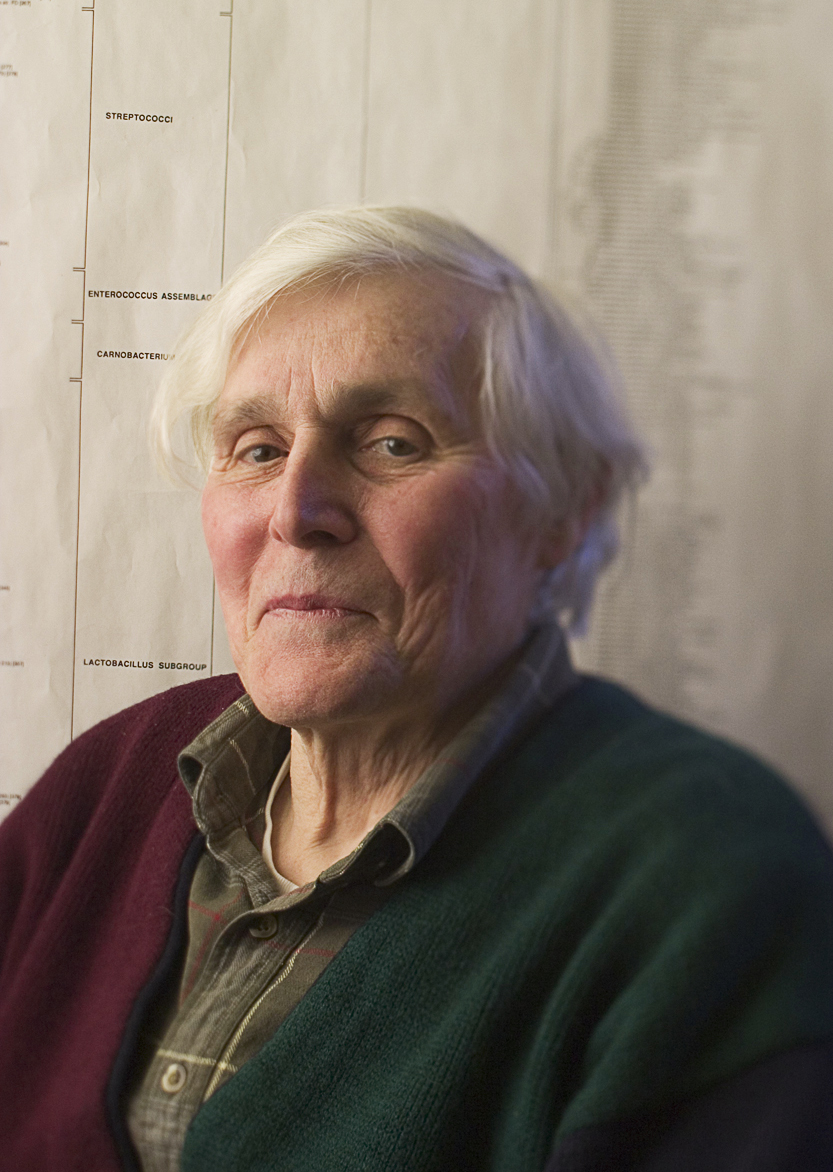
\includegraphics[width=0.34\linewidth]{images/book3/woese.jpg}

{\small Carl Woese (1928--2012), voor een boom van de bacteriën op grond van
\omterm{def:b1:nucleic-acids:rnas}{ribosomaal RNA}. Zijn vergelijking van dit ene molecuul over al het leven
onthulde de Archaea en gaf de levensboom zijn drie domeinen.}
\end{omfigure}

\begin{proposition}[De belangrijkste eukaryotenlijnen]\label{prop:b1:classifying-biodiversity:eukaryotes}
De eukaryoten vallen uiteen in enkele grote groepen: de \emph{opisthokonten}
(dieren, schimmels en hun eencellige verwanten, waarvan de \omterm{def:b1:cell-unit-of-life:cell}{cellen} met één
achterwaartse zweepstaart zwemmen); de \emph{Archaeplastida} (landplanten,
groene en rode algen, met de primaire chloroplast); de \emph{Amoebozoa}; de
\emph{Excavata} (zweepdiertjes als \emph{Trypanosoma} en \emph{Euglena}); en
de \emph{SAR}-groep (stramenopielen als kiezelwieren en bruinwieren;
alveolaten als ciliaten, dinoflagellaten en de malariaparasiet; rhizariën als
foraminiferen en radiolariën). Dieren en schimmels staan dus dichter bij
elkaar dan elk van beide bij de planten; de ``algen'' liggen verspreid over
vier groepen; en de microscopische meerderheid van de eukaryotendiversiteit
ligt buiten de drie rijken met alledaagse namen.
\end{proposition}

\begin{omfigure}
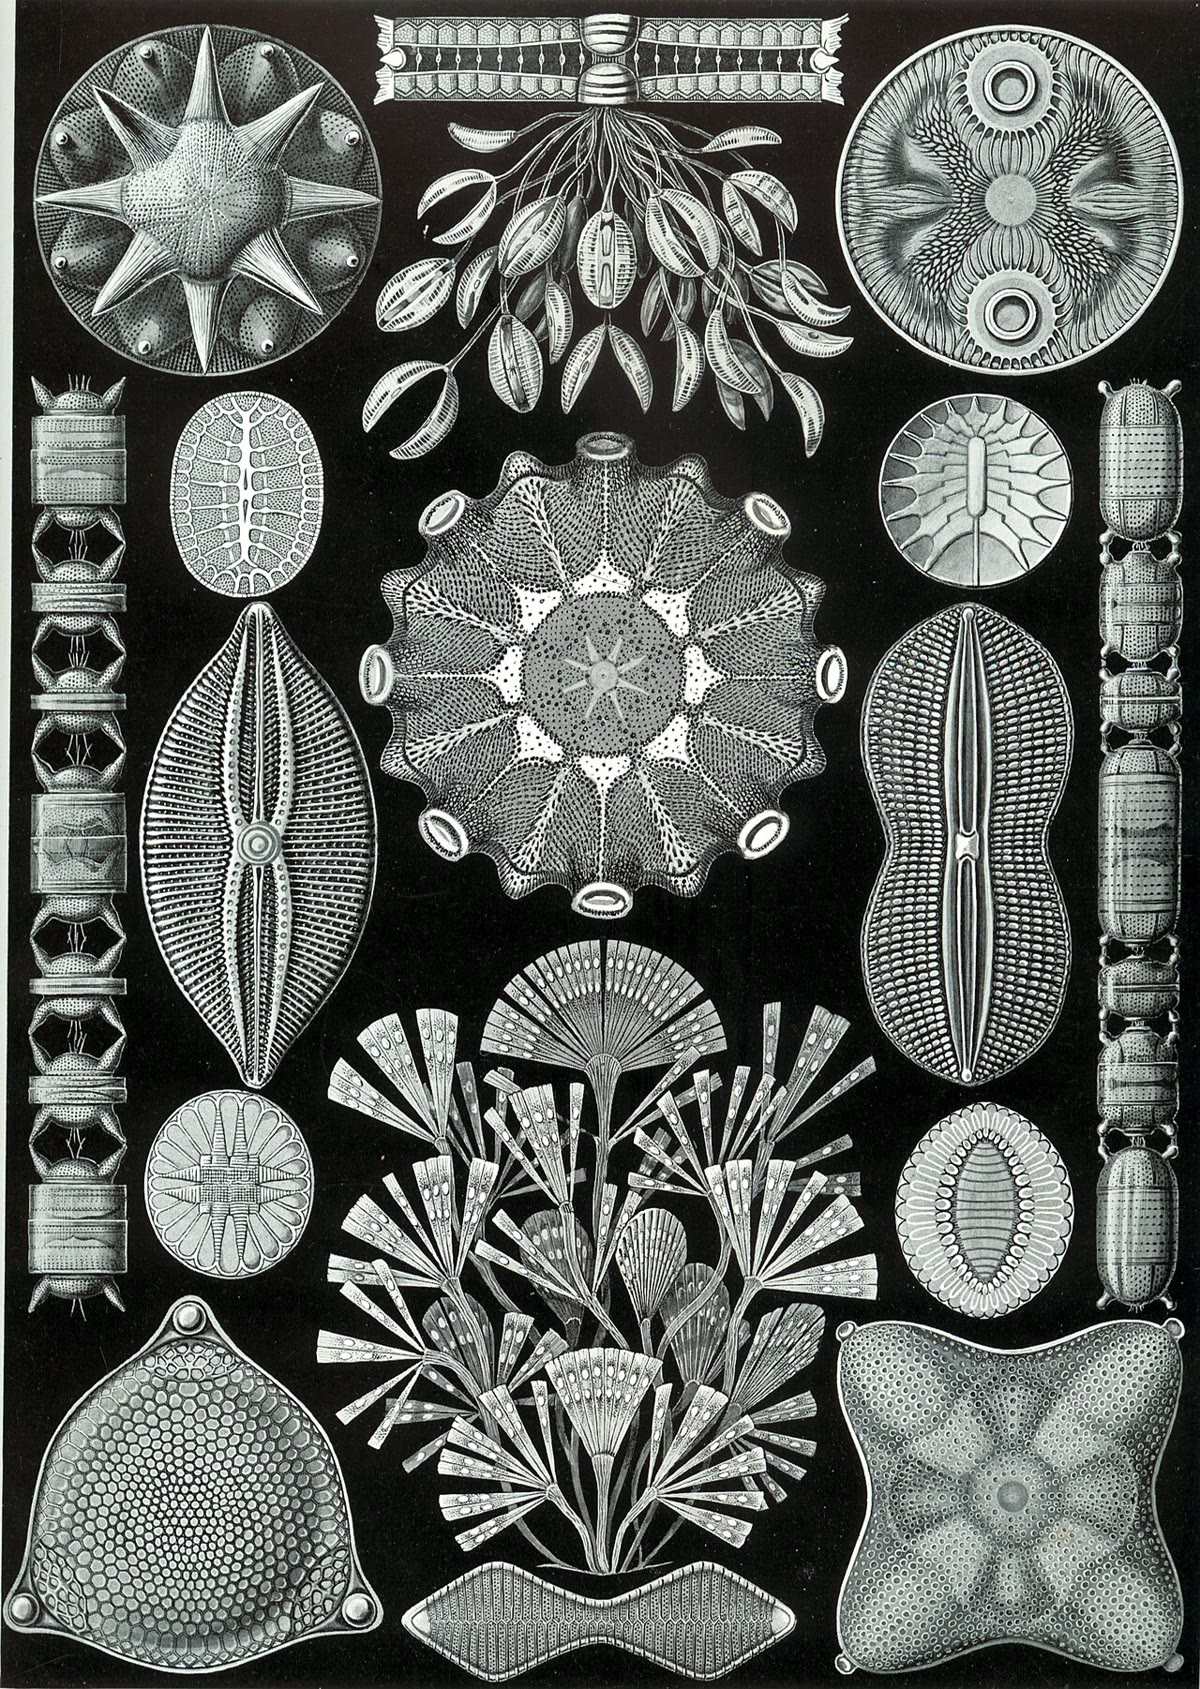
\includegraphics[width=0.36\linewidth]{images/book3/haeckel-diatomea.jpg}\hspace{0.03\linewidth}
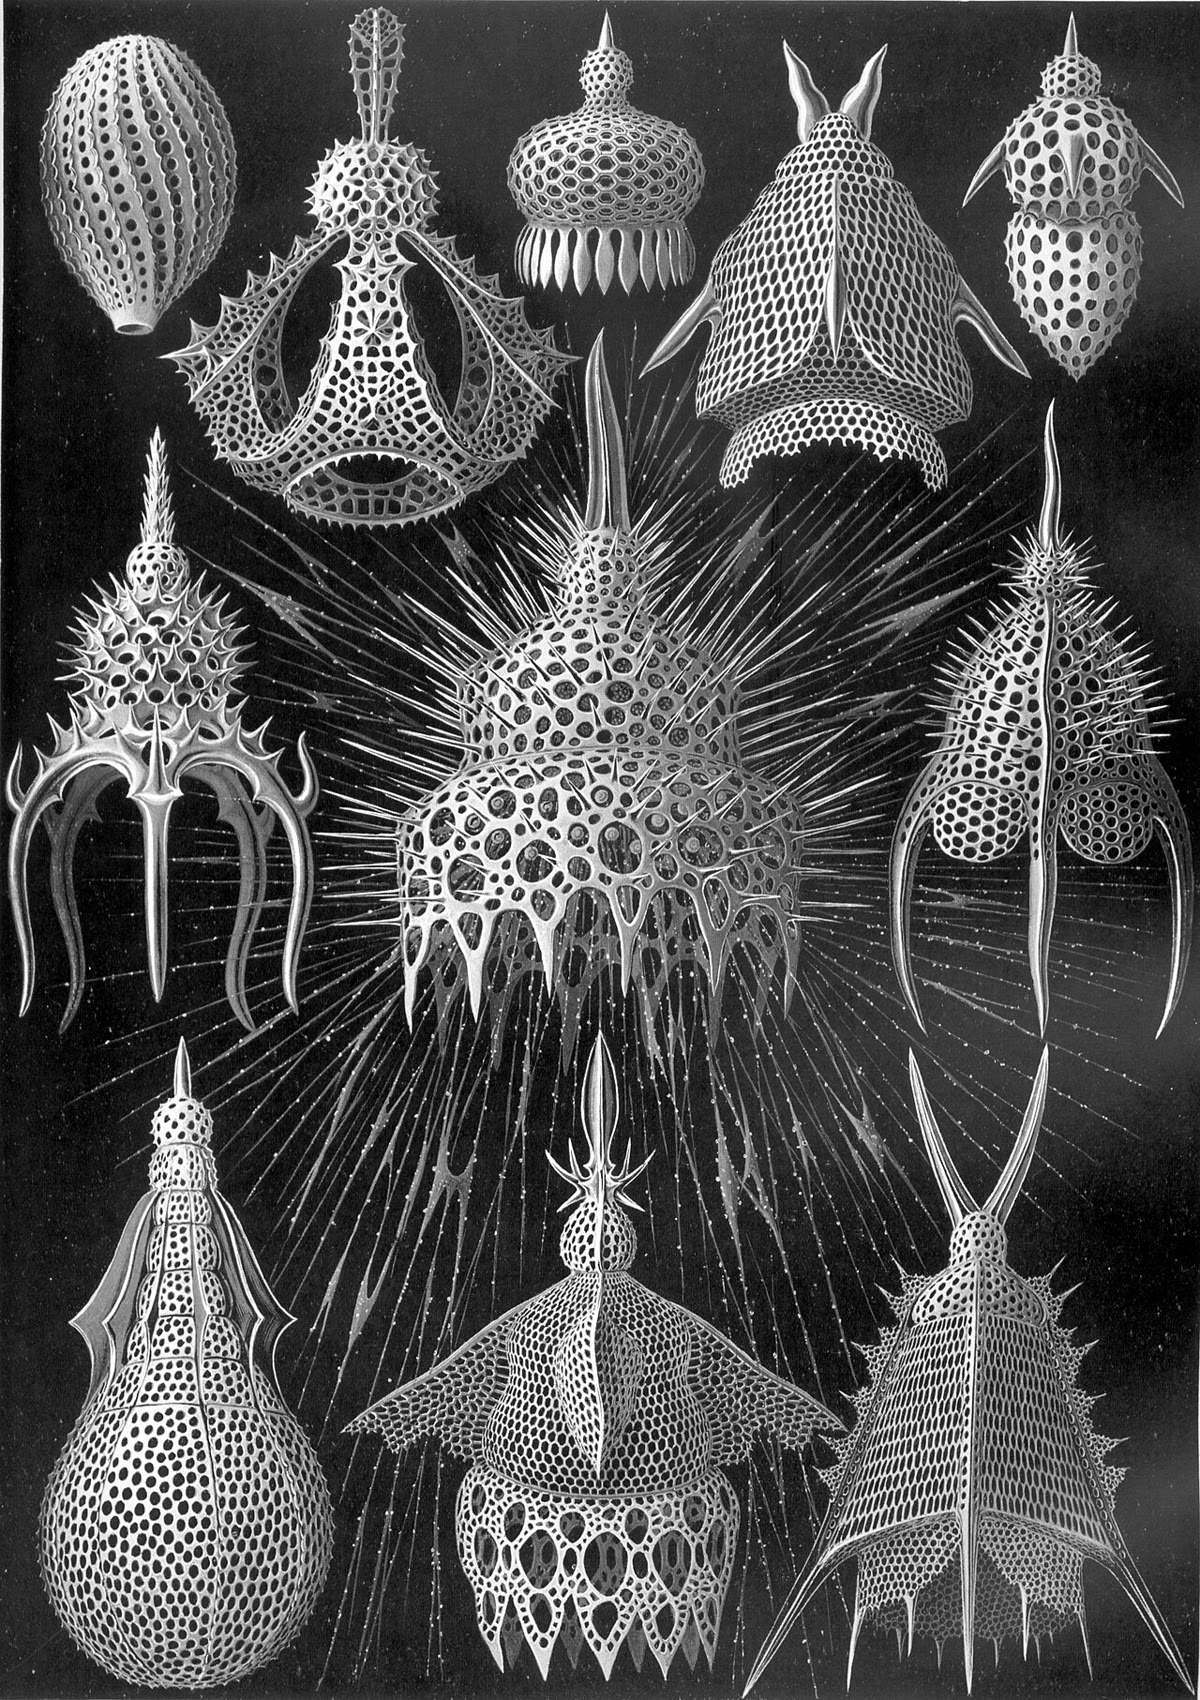
\includegraphics[width=0.36\linewidth]{images/book3/haeckel-cyrtoidea.jpg}

{\small Twee van de eukaryotenlijnen zonder alledaagse naam, op de platen van
Ernst Haeckel uit 1904: kiezelwieren (stramenopielen, in schaaltjes van
kiezel) en radiolariën (rhizariën, in skeletten van kiezel). Elke groep telt
tienduizenden \omterm{def:b1:classifying-biodiversity:species}{soorten}.}
\end{omfigure}

\section{De inventaris van het leven}

\begin{definition}[Biodiversiteit]\label{def:b1:classifying-biodiversity:biodiversity}
\index{biodiversiteit}\index{uitsterven}
\emph{Biodiversiteit} is de verscheidenheid van het leven op elk niveau: de
genetische verscheidenheid binnen \omterm{def:b1:classifying-biodiversity:species}{soorten}, het aantal en de talrijkheid van
de \omterm{def:b1:classifying-biodiversity:species}{soorten}, en de verscheidenheid van \omterm{def:b1:ecosystem-organization:ecosystem}{levensgemeenschappen} en \omterm{def:b1:ecosystem-organization:ecosystem}{ecosystemen}. De
inventaris ervan is onvoltooid: er zijn zo'n \num{2} miljoen \omterm{def:b1:classifying-biodiversity:species}{soorten}
beschreven, waarvan een miljoen insecten, \num{380000} planten,
\num{150000} schimmels, \num{70000} gewervelden en enkele tienduizenden elk
van weekdieren, kreeftachtigen, protisten en prokaryoten; het aantal
eukaryotensoorten wordt, uit het tempo waarin er nog steeds nieuwe hogere
\omterm{def:b1:classifying-biodiversity:nomenclature}{taxa} worden gevonden, op bijna \num{9} miljoen geschat, zodat de meeste
\omterm{def:b1:classifying-biodiversity:species}{soorten} naamloos zijn, en de meeste daarvan klein, tropisch of beide. \omterm{def:b1:classifying-biodiversity:species}{Soorten}
zijn altijd \emph{uitgestorven} --- het achtergrondtempo is volgens de
fossielen ongeveer één \omterm{def:b1:classifying-biodiversity:species}{soort} per miljoen per jaar --- en het huidige tempo,
gedreven door het verlies van \omterm{def:b1:ecosystem-organization:niche}{leefgebied}, overexploitatie, invasieve \omterm{def:b1:classifying-biodiversity:species}{soorten}
en het klimaat, wordt op honderd tot duizend keer zoveel geschat.
\end{definition}

\begin{omfigure}
\begin{tikzpicture}
\begin{axis}[
  xbar, bar width=7pt,
  width=0.82\linewidth, height=6.8cm,
  axis x line=bottom, axis y line=left,
  xmin=0, xmax=1200, xlabel={beschreven soorten (duizenden)},
  xlabel style={font=\small, at={(axis description cs:0.5,-0.12)}, anchor=north},
  symbolic y coords={prokaryoten, zoogdieren, vogels, vissen, protisten, weekdieren, kreeftachtigen, spinachtigen, schimmels, landplanten, insecten},
  ytick=data, tick label style={font=\small},
  enlarge y limits=0.06, xtick={0,200,400,600,800,1000},
  nodes near coords, nodes near coords style={font=\scriptsize, anchor=west},
]
\addplot[fill=omDef!40, draw=omDef] coordinates {(12,prokaryoten) (6.5,zoogdieren) (11,vogels) (35,vissen) (60,protisten) (85,weekdieren) (70,kreeftachtigen) (110,spinachtigen) (150,schimmels) (380,landplanten) (1000,insecten)};
\end{axis}
\end{tikzpicture}

{\small Beschreven \omterm{def:b1:classifying-biodiversity:species}{soorten} per groep, in duizenden (afgerond). De helft van
alle benoemde \omterm{def:b1:classifying-biodiversity:species}{soorten} zijn insecten, en de prokaryoten --- naar elke
moleculaire maat de meest diverse \omterm{def:b1:organism-environment:organism}{organismen} --- hebben minder beschreven
\omterm{def:b1:classifying-biodiversity:species}{soorten} dan de zoogdieren en de vogels samen.}
\end{omfigure}

\begin{omfigure}
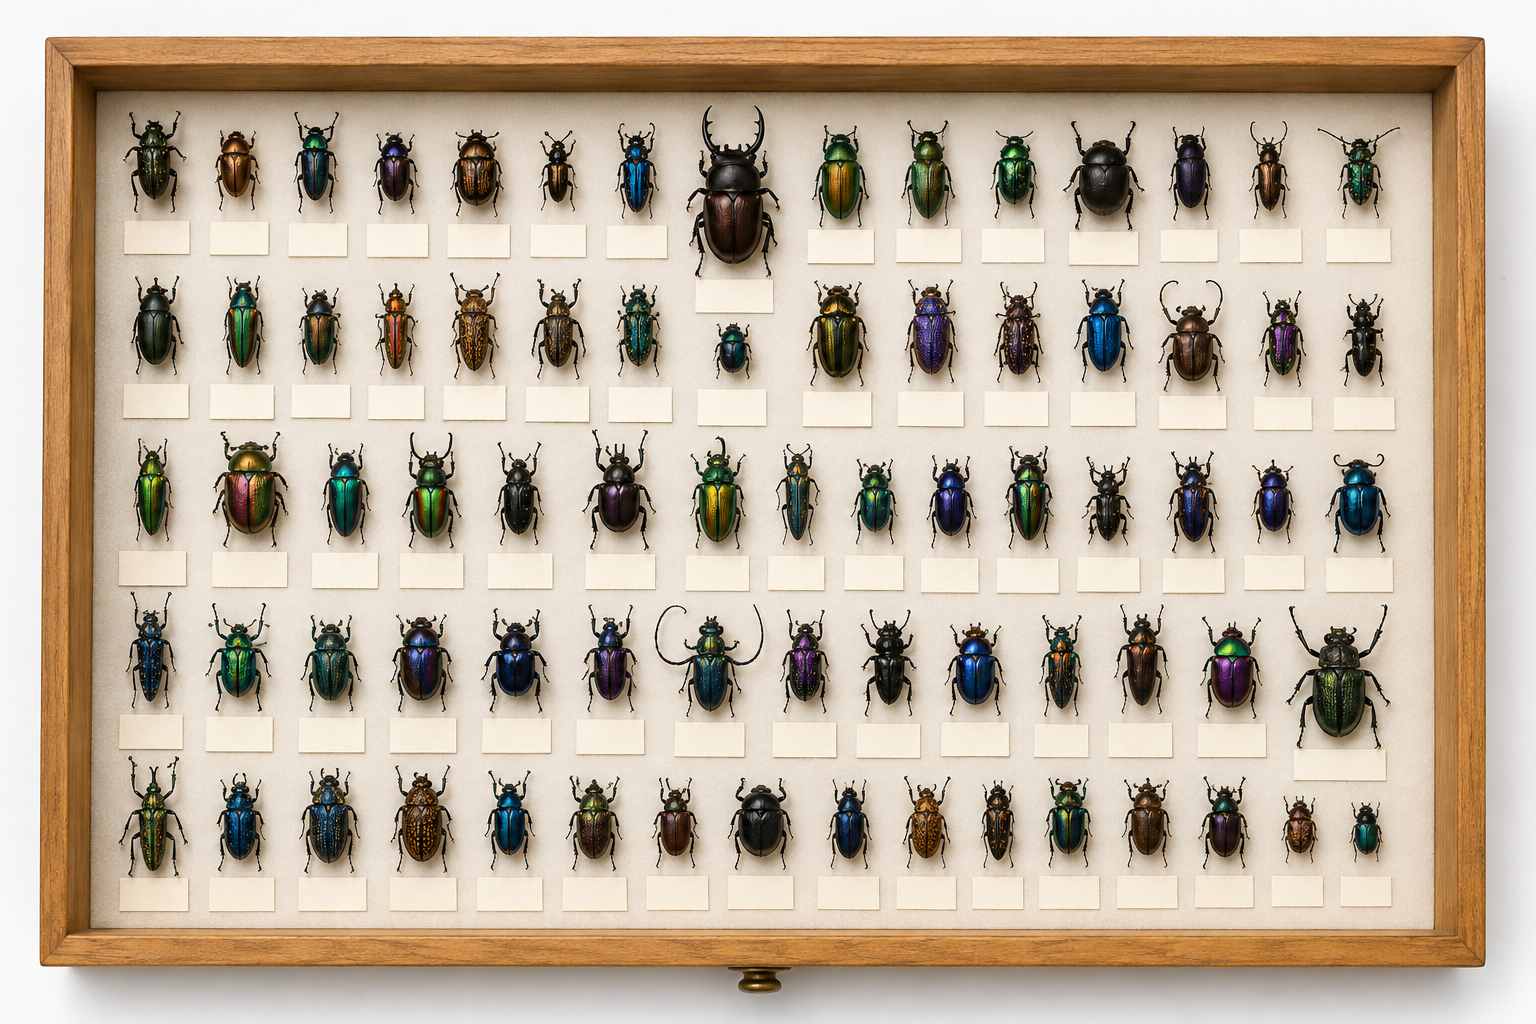
\includegraphics[width=0.56\linewidth]{images/book3/ai/b3-29-beetle-collection.png}

{\small Een museumlade met opgeprikte kevers: de verzameling is de
inventaris, en een lade als deze kan \omterm{def:b1:classifying-biodiversity:species}{soorten} bevatten die nog niemand heeft
benoemd.}
\end{omfigure}

\begin{method}[Schatten hoeveel soorten er zijn]\label{met:b1:classifying-biodiversity:estimate}
\begin{enumerate}
  \item Tel de \omterm{def:b1:classifying-biodiversity:species}{soorten} die in een groep zijn beschreven en het tempo
        waarin er nog nieuwe bij komen; vertraagt dat tempo niet, dan is
        de inventaris nog lang niet volledig.
  \item Extrapoleer van een goed bekende groep naar een slecht bekende
        met een verhouding: als de gematigde faunas twee insectensoorten
        per plantensoort tellen, en de tropen \num{250000} planten
        hebben, tellen de tropen minstens een half miljoen insecten.
  \item Bemonster een klein gebied intensief (een tropische boomkruin met
        insecticide benevelen, het \omterm{def:b1:nucleic-acids:chain}{DNA} van een liter zeewater aflezen) en
        schaal op vanuit het deel van de \omterm{def:b1:classifying-biodiversity:species}{soorten} dat nieuw is.
  \item Gebruik het patroon over de rangen: de aantallen stammen,
        klassen, orden en families zijn vrijwel volledig en stijgen
        regelmatig naar het soortsniveau toe; het doortrekken van die
        regelmaat geeft het totaal (ongeveer \num{8.7} miljoen
        eukaryoten).
  \item Meld de schatting met haar marge; het eerlijke antwoord voor de
        prokaryoten is een marge van verscheidene ordes van grootte.
\end{enumerate}
\end{method}

\section{Exercises}

\begin{exercise}[$\star$]\label{exo:b1:classifying-biodiversity:1}
Schrijf de naam van de huiskat correct op, benoem haar \omterm{def:b1:classifying-biodiversity:nomenclature}{geslacht} en
soortaanduiding, en plaats haar in haar familie, orde, klasse en stam.
\end{exercise}

\begin{exercise}[$\star$]\label{exo:b1:classifying-biodiversity:2}
Omschrijf \omterm{def:b1:classifying-biodiversity:characters}{homologie} en \omterm{def:b1:classifying-biodiversity:characters}{homoplasie} met van elk een voorbeeld, en zeg welke van
beide bewijs voor een \omterm{def:b1:classifying-biodiversity:systematics}{clade} is.
\end{exercise}

\begin{exercise}[$\star$]\label{exo:b1:classifying-biodiversity:3}
Zeg of ``vissen'', ``vogels'' en ``warmbloedige dieren'' monofyletisch,
parafyletisch of polyfyletisch zijn, met de reden erbij.
\end{exercise}

\begin{exercise}[$\star$]\label{exo:b1:classifying-biodiversity:4}
Noem de drie domeinen en geef twee eigenschappen die de Archaea van de
Bacteria scheiden.
\end{exercise}

\begin{exercise}[$\star\star$]\label{exo:b1:classifying-biodiversity:5}
Waarom kan het biologische soortsbegrip niet op bacteriën of op fossielen
worden toegepast, en wat wordt er in de plaats gebruikt?
\end{exercise}

\begin{exercise}[$\star\star$]\label{exo:b1:classifying-biodiversity:6}
Drie \omterm{def:b1:classifying-biodiversity:nomenclature}{taxa} X, Y, Z en een \omterm{def:b1:classifying-biodiversity:characters}{buitengroep}. Kenmerk 1 is afgeleid bij X en Y;
kenmerk 2 bij Y en Z; kenmerk 3 bij X en Y; kenmerk 4 bij X en Y. Teken de
twee mogelijke bomen, bereken hun lengten, en geef de spaarzaamste boom en
zijn \omterm{def:b1:classifying-biodiversity:characters}{homoplasie}.
\end{exercise}

\begin{exercise}[$\star\star$]\label{exo:b1:classifying-biodiversity:7}
Waarom is er een \omterm{def:b1:classifying-biodiversity:characters}{buitengroep} nodig om een cladogram te bouwen, en wat gaat er
mis als de gekozen \omterm{def:b1:classifying-biodiversity:characters}{buitengroep} in werkelijkheid binnen de groep hoort?
\end{exercise}

\begin{exercise}[$\star\star$]\label{exo:b1:classifying-biodiversity:8}
Leg uit waarom dieren en schimmels als nauwere verwanten worden beschouwd dan
dieren en planten, en welk kenmerk de opisthokonten delen.
\end{exercise}

\begin{exercise}[$\star\star$]\label{exo:b1:classifying-biodiversity:9}
Woese vond dat methanogenen even sterk van de overige bacteriën verschillen
als van de eukaryoten. Waarom rechtvaardigde dat een nieuw domein en niet een
nieuw rijk binnen de bacteriën?
\end{exercise}

\begin{exercise}[$\star\star\star$]\label{exo:b1:classifying-biodiversity:10}
Een tropische boomkruin die met insecticide is beneveld levert 1200
keversoorten op, waarvan \qty{20}{\%} eigen is aan die boomsoort; kevers zijn
\qty{40}{\%} van de insecten van de kruin, en de kruin herbergt twee derde
van de insecten van de boom; er zijn \num{50000} tropische boomsoorten. Schat
het aantal tropische insectensoorten en noem de aannamen.
\end{exercise}

\begin{exercise}[$\star\star\star$]\label{exo:b1:classifying-biodiversity:11}
Een \omterm{def:b1:classifying-biodiversity:species}{soort} wordt van één enkel museumexemplaar beschreven; later worden er
levende \omterm{def:b1:populations:population}{populaties} gevonden die er iets van verschillen. Leg de rol van het
\omterm{def:b1:classifying-biodiversity:nomenclature}{typemateriaal} uit bij het bepalen waarop de naam van toepassing is, en waarom
voorrang ertoe doet.
\end{exercise}

\begin{exercise}[$\star\star\star$]\label{exo:b1:classifying-biodiversity:12}
``\omterm{def:b1:classifying-biodiversity:parsimony}{Spaarzaamheid} veronderstelt dat de evolutie de kortste weg neemt.''
Bespreek dat: wat \omterm{def:b1:classifying-biodiversity:parsimony}{spaarzaamheid} wel veronderstelt, wanneer zij faalt
(convergentie, snel evoluerende lijnen), en hoe moleculaire gegevens en
fossielen worden gebruikt om een boom te toetsen.
\end{exercise}

\section{Vraagstuk: acht gewervelden en een boom}

\begin{problem}[{Weekendvraagstuk --- een kenmerkmatrix van acht gewervelden,
haar cladogram met de hand gebouwd, twee rivaliserende bomen op
spaarzaamheid beoordeeld, de overgeleverde groepen op monofylie getoetst, en
een schatting van het aantal soorten, eindigend op de spaarzaamste boom en
zijn lengte}]
\label{pb:b1:classifying-biodiversity:1}
De matrix scoort tien kenmerken (1 = afgeleide toestand aanwezig) voor een
prik (\omterm{def:b1:classifying-biodiversity:characters}{buitengroep}), een haai, een forel, een longvis, een kikker, een
hagedis, een muis en een duif.

\begin{center}
\footnotesize
\begin{tabular}{l*{10}{c}}
\hline
 & 1 & 2 & 3 & 4 & 5 & 6 & 7 & 8 & 9 & 10 \\
 & \rotatebox{90}{kaken} & \rotatebox{90}{benig \omterm{def:b1:body-plans-tissues:segments}{skelet}} & \rotatebox{90}{\omterm{def:b1:gas-exchange:lung}{longen}} & \rotatebox{90}{vier ledematen} & \rotatebox{90}{amnionei} & \rotatebox{90}{haren} & \rotatebox{90}{veren} & \rotatebox{90}{diapside schedel} & \rotatebox{90}{endothermie} & \rotatebox{90}{keratineschubben} \\
\hline
prik & 0 & 0 & 0 & 0 & 0 & 0 & 0 & 0 & 0 & 0 \\
haai & 1 & 0 & 0 & 0 & 0 & 0 & 0 & 0 & 0 & 0 \\
forel & 1 & 1 & 0 & 0 & 0 & 0 & 0 & 0 & 0 & 0 \\
longvis & 1 & 1 & 1 & 0 & 0 & 0 & 0 & 0 & 0 & 0 \\
kikker & 1 & 1 & 1 & 1 & 0 & 0 & 0 & 0 & 0 & 0 \\
hagedis & 1 & 1 & 1 & 1 & 1 & 0 & 0 & 1 & 0 & 1 \\
muis & 1 & 1 & 1 & 1 & 1 & 1 & 0 & 0 & 1 & 0 \\
duif & 1 & 1 & 1 & 1 & 1 & 0 & 1 & 1 & 1 & 1 \\
\hline
\end{tabular}
\end{center}

\medskip
\noindent\textbf{Deel I --- De matrix lezen.}
\begin{enumerate}
  \item Welke kenmerken worden door alle \omterm{def:b1:classifying-biodiversity:nomenclature}{taxa} behalve de \omterm{def:b1:classifying-biodiversity:characters}{buitengroep}
        gedeeld? Wat vertellen zij over de boom?
  \item Zet de kenmerken op volgorde van het aantal \omterm{def:b1:classifying-biodiversity:nomenclature}{taxa} dat de afgeleide
        toestand deelt, en zeg welke \omterm{def:b1:classifying-biodiversity:systematics}{clade} elk kenmerk bepaalt.
  \item Welke kenmerken komen bij één enkel \omterm{def:b1:classifying-biodiversity:nomenclature}{taxon} voor? Zijn zij van enig
        nut bij het plaatsen van dat \omterm{def:b1:classifying-biodiversity:nomenclature}{taxon}?
  \item Welk paar kenmerken botst met elkaar, en tussen welke drie \omterm{def:b1:classifying-biodiversity:nomenclature}{taxa}?
  \item Geef de polariteit van kenmerk 3 (\omterm{def:b1:gas-exchange:lung}{longen}) en leg uit hoe de
        \omterm{def:b1:classifying-biodiversity:characters}{buitengroep} die vastlegt.
  \item Hoeveel verschillende gewortelde bomen kunnen de drie amnioten met
        elkaar verbinden, als de rest van de boom vastligt? Welke
        kenmerken zijn van belang voor de keuze?
\end{enumerate}

\medskip
\noindent\textbf{Deel II --- De boom bouwen.}
\begin{enumerate}[resume]
  \item Teken het cladogram dat uit de kenmerken 1 tot en met 5 volgt: de
        geneste \omterm{def:b1:classifying-biodiversity:systematics}{claden} van kaken tot het amnionei.
  \item Teken binnen de amnioten boom A, waarin de hagedis en de duif
        zustertaxa zijn, en boom B, waarin de muis en de duif zusters
        zijn.
  \item Bereken de lengte van boom A: voor elk van de tien kenmerken het
        kleinste aantal veranderingen dat het vraagt.
  \item Bereken op dezelfde wijze de lengte van boom B.
  \item Welke boom is de spaarzaamste, en met hoeveel?
  \item Noem het homoplastische kenmerk op de gekozen boom en beschrijf de
        evolutionaire duiding ervan.
  \item Wat zouden de twee lengten zijn als de kenmerken 8 en 10 werden
        weggelaten, en wat zou daaruit volgen?
\end{enumerate}

\medskip
\noindent\textbf{Deel III --- Groepen op de boom.}
\begin{enumerate}[resume]
  \item Is de groep (haai, forel, longvis) --- de ``vissen'' --- op de
        gekozen boom monofyletisch? Welk \omterm{def:b1:classifying-biodiversity:nomenclature}{taxon} zou eraan moeten worden
        toegevoegd?
  \item Is (hagedis, muis, duif), de amnioten, monofyletisch? Noem haar
        \omterm{def:b1:classifying-biodiversity:characters}{synapomorfie}.
  \item Is (hagedis) alleen plus de krokodillen en de schildpadden --- de
        overgeleverde ``reptielen'' --- monofyletisch zodra de duif is
        geplaatst? Wat voor type groep is dat?
  \item Is (muis, duif), samengebracht op endothermie, een \omterm{def:b1:classifying-biodiversity:systematics}{clade}? Wat voor
        \omterm{def:b1:classifying-biodiversity:species}{soort} groep is dat?
  \item De longvis wordt vaak een vis genoemd. Staat hij op de boom
        dichter bij de forel of bij de kikker? Welk kenmerk beslist?
  \item Geef de rangen die de drie amnioten in een indeling volgens
        Linnaeus zouden innemen, en leg uit waarom de rangen niets zeggen
        over de diepte van hun splitsingen.
\end{enumerate}

\medskip
\noindent\textbf{Deel IV --- De inventaris.}
\begin{enumerate}[resume]
  \item Er zijn ongeveer \num{70000} \omterm{def:b1:classifying-biodiversity:species}{soorten} gewervelden beschreven en het
        tempo van nieuwe beschrijvingen is \num{300} per jaar voor vissen
        en \num{20} voor zoogdieren. Welke inventaris is het dichtst bij
        voltooiing?
  \item Een verkenning van het \omterm{def:b1:nucleic-acids:chain}{DNA} in \qty{1}{L} zeewater vindt
        \num{2000} verschillende ribosomale volgorden, waarvan
        \qty{90}{\%} met geen enkel beschreven \omterm{def:b1:organism-environment:organism}{organisme} overeenkomt. Wat
        houdt dat in voor de inventaris van de prokaryoten?
  \item Als het achtergrondtempo van \omterm{def:b1:classifying-biodiversity:biodiversity}{uitsterven} één \omterm{def:b1:classifying-biodiversity:species}{soort} per miljoen per
        jaar is en er \num{9} miljoen eukaryotensoorten zijn, hoeveel
        zouden er dan per jaar moeten \omterm{def:b1:classifying-biodiversity:biodiversity}{uitsterven}? Het waargenomen tempo
        voor goed bestudeerde groepen ligt ongeveer \num{1000} keer
        hoger: hoeveel per jaar geeft dat voor alle eukaryoten?
  \item Waarom is een \omterm{def:b1:classifying-biodiversity:species}{soort} die uitsterft voordat zij is beschreven
        evenzeer een verlies voor de \omterm{def:b1:classifying-biodiversity:systematics}{systematiek} als voor het \omterm{def:b1:ecosystem-organization:ecosystem}{ecosysteem}?
  \item Leg uit waarom het aantal beschreven families een betere maat voor
        het totaal is dan het aantal beschreven \omterm{def:b1:classifying-biodiversity:species}{soorten}.
  \item Geef het resultaat: de spaarzaamste boom van de acht gewervelden,
        in geneste haakjes geschreven, en zijn lengte.
\end{enumerate}
\end{problem}
